\chapter{IMPLEMENTATION AND TESTING}
\section{Implementation}
"Code Connect" is a delightful online space where programmers come together to share ideas and experiences. Using tools like HTML, CSS, and JavaScript, we've built a website that's easy to use and fun to explore. Behind the scenes, PHP and MySQL work like magic to handle all the information. With AJAX and JQuery, everything feels smooth and interactive, just like chatting with friends. It's not just about technology – it's about people connecting and learning from each other. Just like baking a tasty treat, we've mixed all these ingredients to create something special that everyone can enjoy.


% (20\% of Report Length)

% a. Showcase the output at various intermediate stages of the project pipeline

% b. Use proper data visualizing techniques to present the output

% c. Figures and tables must be accompanied by an explanation
\section{Tools Used}
\subsection{Git}
Git is a version control system essential for software development and collaborative projects. It efficiently manages changes to files by recording them as "commits," enabling easy tracking and reverting to previous versions. Git's power lies in fostering collaboration, allowing multiple individuals to work on projects simultaneously through branches. These branches facilitate independent development, and Git's merging capabilities seamlessly integrate diverse changes into the main codebase. Its historical recording acts as a backup and recovery mechanism, safeguarding against data loss. Moreover, Git promotes code reviews, enabling precise feedback on proposed changes, and enhancing overall code quality. The isolation of work in separate branches reduces conflicts and enhances focus. It's especially popular in the open-source community, aiding global contributors to collaborate via forks and pull requests. Git's integration with CI/CD pipelines automates testing and deployment, making it an integral part of modern development processes. In essence, Git empowers teams with version control, collaboration tools, and an efficient system to manage changes, fostering productive and streamlined project development.
\subsection{Figma}
Figma is a cloud-based design and prototyping tool widely used for creating user interfaces and interactive designs for web and mobile applications. Its standout feature is real-time collaboration, allowing multiple users to work simultaneously on the same design, fostering seamless teamwork. With versatile design tools encompassing vector editing, typography controls, and color management, Figma empowers designers to craft intricate layouts and visually appealing interfaces. Interactive prototypes can be developed with clickable elements, animations, and transitions, aiding in simulating user interactions and presenting functionality. Component and style libraries ensure design consistency and efficiency, while design handoff is simplified through easy sharing of specs, assets, and CSS properties. Figma promotes stakeholder engagement by facilitating user testing and feedback collection within the platform. It extends its functionality through a wide range of plugins and integrates with various design and development tools, accommodating diverse workflows. Cross-platform compatibility, version history, and undo capabilities contribute to a flexible and efficient design process. Overall, Figma's collaborative, versatile, and user-centric features make it a valuable asset for teams aiming to deliver compelling digital experiences.
\subsection{GitHub}
GitHub is a web-based platform pivotal to software development, offering version control and collaboration tools. It employs Git for version control, tracing code changes and preventing conflicts, while hosting repositories to centralize code storage and collaboration. Through collaborative development, multiple developers can work concurrently on a project, making changes in separate branches and merging them into the main codebase. Pull requests enable proposed changes to undergo review and discussion before integration, ensuring code accuracy. An integrated issue tracker handles bug reports, feature suggestions, and project discussions, while wikis and documentation enhance accessibility. GitHub seamlessly integrates with CI/CD tools for automated testing and deployment. Popular in the open-source realm, it encourages community participation by enabling contributions and project forks. Security measures include vulnerability scanning and permissions management. In essence, GitHub serves as a collaborative hub for version control, code management, issue tracking, and community involvement, empowering efficient, high-quality software development.
\subsection{HTML, CSS and JS}
\begin{itemize}
    \item \textbf{HTML (Hypertext Markup Language)}: HTML is the foundational language used to create the structure of web content. It uses a system of tags to define elements like headings, paragraphs, links, images, and more. These tags give structure to web pages, organizing content into a meaningful layout. HTML provides the framework for displaying information and forming the basis for user interaction on the web.

    \item \textbf{CSS (Cascading Style Sheets)}: CSS is a styling language that complements HTML by controlling the visual presentation of web content. It allows developers to define colors, fonts, margins, borders, and other design aspects of HTML elements. By separating content from presentation, CSS enables consistent styling across web pages and enhances user experience through improved aesthetics and readability.

    \item \textbf{JavaScript (JS)}: JavaScript is a versatile scripting language used to add interactivity and dynamic behavior to web pages. It enables developers to create responsive features such as form validation, animations, pop-ups, and real-time updates. JS executes directly in the browser, allowing users to interact with web content without requiring page reloads. It's a crucial component for creating engaging and interactive web experiences.

\end{itemize}
\subsection{MySQL}
MySQL is an amazing open-source relational database management system (RDBMS) that's super popular for organizing and handling structured data like a pro. It's like a superhero for managing loads of information, whether you're building websites or business tools. The cool thing is that MySQL speaks a special language called SQL (Structured Query Language), which lets you create, tweak, and ask questions about databases. You can set up tables, make connections between data, and do fancy searches with ease. It's got your back with features like making sure data is legit, indexing for quick data finding, and even handling transactions so things stay reliable. MySQL's built to let lots of people work on data together, all while keeping things secure and controlled. Whether you're building something small or a massive enterprise project, MySQL's got the chops to handle it all. With its adaptability, community support, and knack for playing nice with other tech, MySQL is your go-to tool for wrangling data and making applications that really work.
\subsection{PHP}
In the realm of web development, PHP emerges as a scripting language that commands attention. As the author of this report, I find myself captivated by PHP's capabilities and its pivotal role in creating dynamic and interactive websites. Picture a scenario where a website needs to process forms, communicate with databases, or display content that adapts to user actions – this is where PHP steps onto the stage. Seamlessly integrated with HTML, PHP empowers websites to exhibit a range of enchanting functionalities. It bestows the power to build responsive forms that wield actual functionality, to interact with databases effortlessly, and to breathe life into web content through dynamic displays that transform in real-time. The beauty of PHP lies in its collaborative spirit; being open-source, it's akin to having a community of like-minded developers ready to offer assistance and guidance. For novices and seasoned developers alike, PHP serves as a formidable tool, amplifying the potential of web projects with its prowess in functionality and innovation. As I delve into the intricacies of PHP, I am compelled to highlight its role as a cornerstone in modern web development, an indispensable asset for crafting websites that stand out in the digital landscape.
\section{Modules Used}
\subsection{AJAX}
In the dynamic realm of web development, AJAX (Asynchronous JavaScript and XML) emerges as a groundbreaking technique that has redefined the way web pages engage with servers to deliver content. As the author of this report, I find myself captivated by the transformative capabilities that AJAX introduces to the digital landscape. With AJAX, the marriage of JavaScript and server communication takes on a new dimension, offering a seamless and asynchronous mode of data exchange. Unlike conventional methods that demand full page reloads to update content, AJAX empowers developers to fetch and transmit data in the background, gracefully refreshing specific sections of a web page without disrupting the user experience. A notable aspect of AJAX is its compatibility with various data formats, such as XML and JSON, which facilitate efficient and reliable data transmission. This versatile technique enables real-time updates, form submissions, and content loading that harmonize with users' actions. In essence, AJAX endows web applications with a dynamic, responsive, and interactive nature that echoes the sophistication of traditional desktop applications, elevating user engagement and propelling the field of modern web development into a new era of possibilities.
\subsection{JQuery}
Embarking on the journey of web development, one encounters jQuery as an influential player that has transformed the way interaction with HTML, CSS, and JavaScript. In the realm of crafting dynamic and interactive web experiences, I am intrigued by the capabilities that jQuery, as a fast, small, and feature-rich JavaScript library, brings to the forefront. As a contributor to this report, I find myself immersed in the profound impact that jQuery has on simplifying complex tasks and enhancing user interaction. By providing a streamlined way to manipulate the Document Object Model (DOM), jQuery empowers developers to effortlessly select, modify, and animate HTML elements. Its user-friendly syntax and extensive range of built-in functions alleviate the challenges posed by cross-browser compatibility issues, allowing seamless development across various platforms. Moreover, jQuery's plugin ecosystem magnifies its potential, offering a plethora of pre-built functionalities that can be easily integrated into projects. The library's essence lies in abstracting intricate JavaScript operations into concise commands, resulting in cleaner code and expedited development cycles. Through its capabilities in event handling, animations, and AJAX requests, jQuery serves as a catalyst for elevating user experiences and accelerating the creation of captivating, feature-rich web applications.
\subsection{MySqli Connect}
In the domain of web development and database connectivity, the mysqli\_connect function emerges as a cornerstone tool that I find fascinating to explore. As the author of this report, I'm intrigued by the pivotal role that mysqli\_connect plays in establishing a seamless link between web applications and MySQL databases. This function, nestled within the PHP programming language, holds the power to initiate secure connections to databases, enabling the retrieval and manipulation of data. By providing parameters such as the database host, username, password, and database name, developers gain the ability to effortlessly establish a communication channel with MySQL servers. This function's significance lies in its contribution to the dynamic generation of interactive web applications, as it forms the foundational bridge for data-driven features and functionalities. With mysqli\_connect, I am captivated by its influence in shaping efficient and responsive web experiences, making it a cornerstone component in the realm of modern database-driven web development.
\subsection{Google Fonts}
In the context of web design and typography exploration, I've had the privilege of discovering the transformative capabilities of Google Fonts. As I delve into this subject for our report, I'm genuinely impressed by the role Google Fonts plays in revolutionizing the way that is approached text presentation on the web. The vast array of fonts available at our fingertips, curated with precision and diversity, has left a lasting impression on me. Google Fonts not only addresses the creative aspirations of designers but also places user experience at the forefront by promoting accessible and visually appealing text choices. With an intuitive interface and seamless integration, the process of embedding selected fonts into projects feels intuitive and user-friendly. The cherry on top is a performance optimization, ensuring that the aesthetic enhancements don't compromise website speed. My exploration of Google Fonts underscores its significance as a valuable asset in the design arsenal, enhancing both the aesthetics and accessibility of web content in a meaningful way.
\subsection{Font Awesome }
Navigating the realm of web design and user interface enhancement, I've been captivated by the remarkable utility that Font Awesome offers. As I delve into the depths of this report, I find myself immersed in the significance of Font Awesome's icon library in modern web development. The array of icons, meticulously crafted and encompassing a wide spectrum of categories, has truly left an impression on me. Font Awesome not only simplifies the process of integrating icons into web projects, but it also adds a layer of visual appeal and functionality that resonates with users. The convenience of using CSS classes to seamlessly incorporate icons and the option to customize their size, color, and style gives designers a dynamic toolbox for creative expression. What intrigues me further is its compatibility with various frameworks and platforms, making it a versatile choice for both beginners and seasoned developers. As I examine the impact of Font Awesome on enhancing user experiences, I'm struck by its ability to add depth and meaning to digital interfaces, making it an indispensable asset in the journey of crafting captivating and user-centric web applications.
% \subsection{Implementation Details of Modules}
% \section{Testing}
% \subsection{Test Cases for Unit Testing}
% \subsection{Test Cases for System Testing}
\section{Testing}
\subsection{Unit Testing}
Unit testing is a software testing technique where individual units or components of a software application are tested in isolation to ensure that they function correctly. These units can be functions, methods, classes, or even small modules. Unit testing aims to verify that each unit performs as expected, providing developers with confidence that their code works as intended and catches bugs early in the development process.
\\
\textbf{Authenication Unit}\\
Here testing different test cases of authentication system in Code Connect is performed with screenshots as required results:\\
\begin{tabular}{|p{0.3in}|p{1.5in}|p{1.5in}|p{1.5in}|}
    \hline
    Tests & Test Cases & Input & Output \\
    \hline
        1 & Incorrect Password& Email:test@gmail.com Password:1234& Incorrect Password \\
        \hline
        2 & Incorrect Confirm Password in SignUp & Email:test@gmail.com
        Password:12345679
        Password:12345678 & Enter Same Password \\
        \hline
        3 & Correct Credentials In Login & Email:test@gmail.com
        Password:12345679 & Redirects to homepage \\
        \hline
\end{tabular}

% \begin{figure}[ht]
%     \centering
%     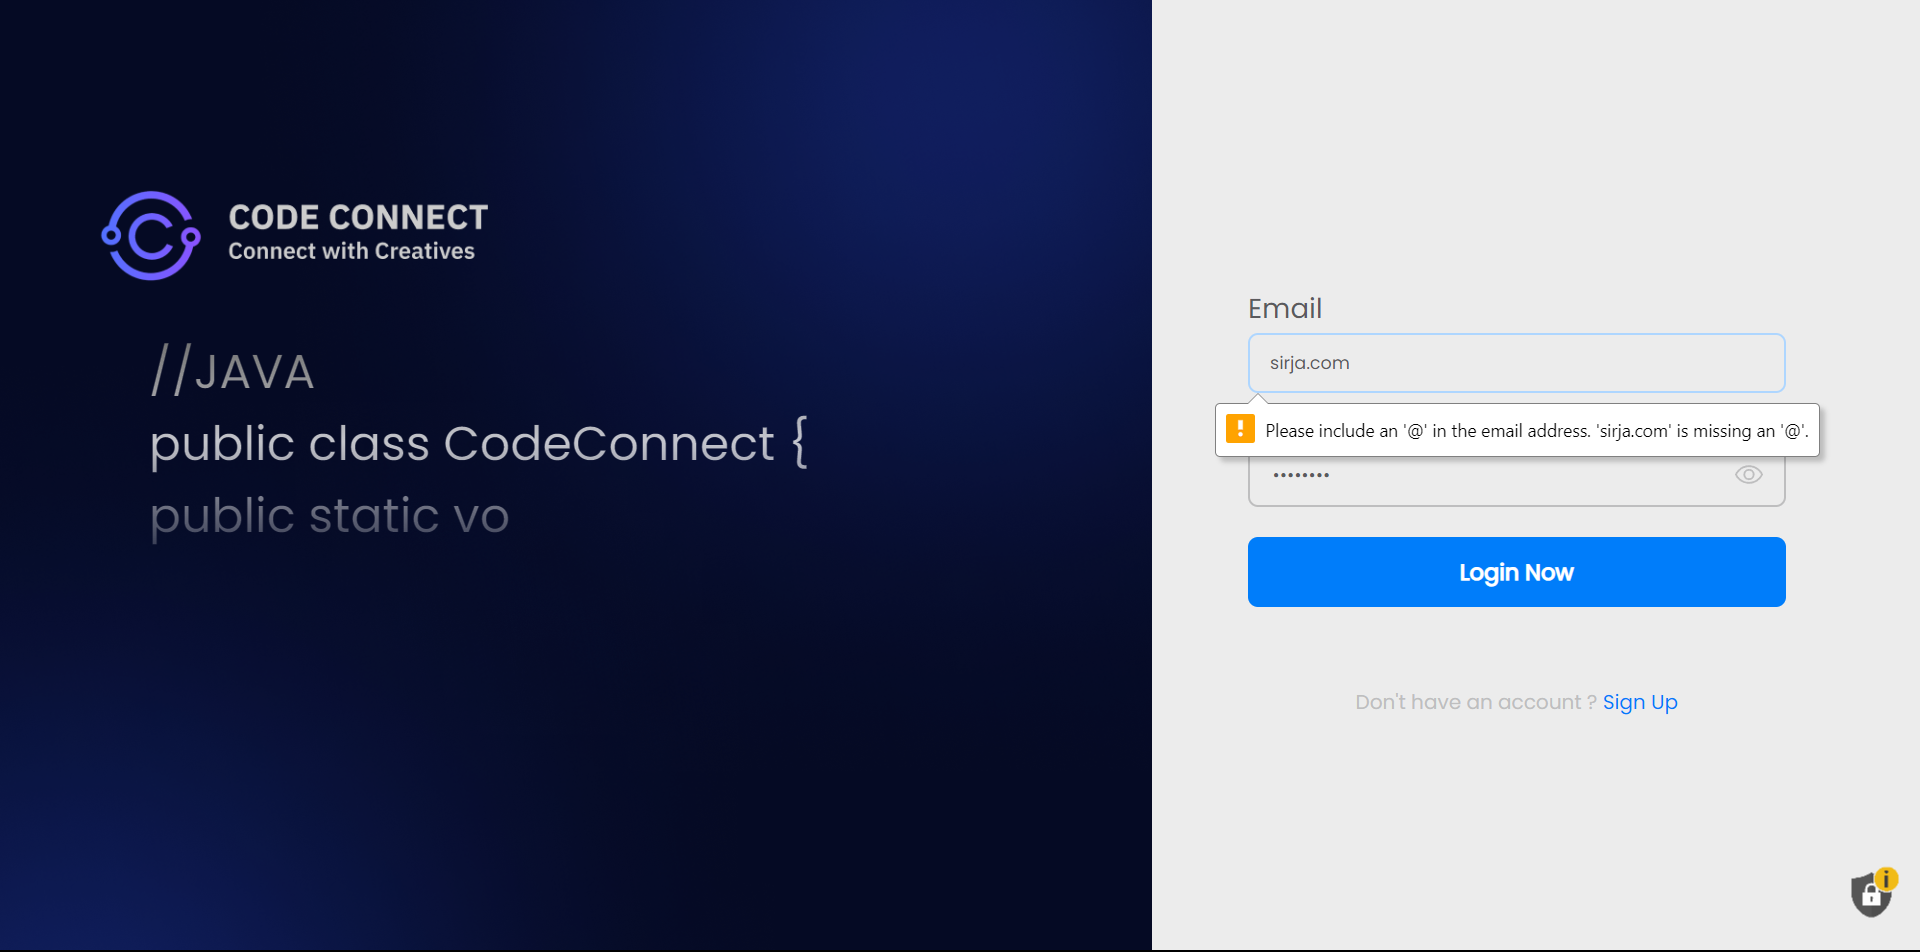
\includegraphics[width=1\textwidth]{4ImplementationAndTesting/screenshots/email-err-signin.png}
%     \caption{Incorrect email Format}
%     \label{fig: Incorrect email Format}

% \end{figure}
% \begin{figure}[ht]
%     \centering
%     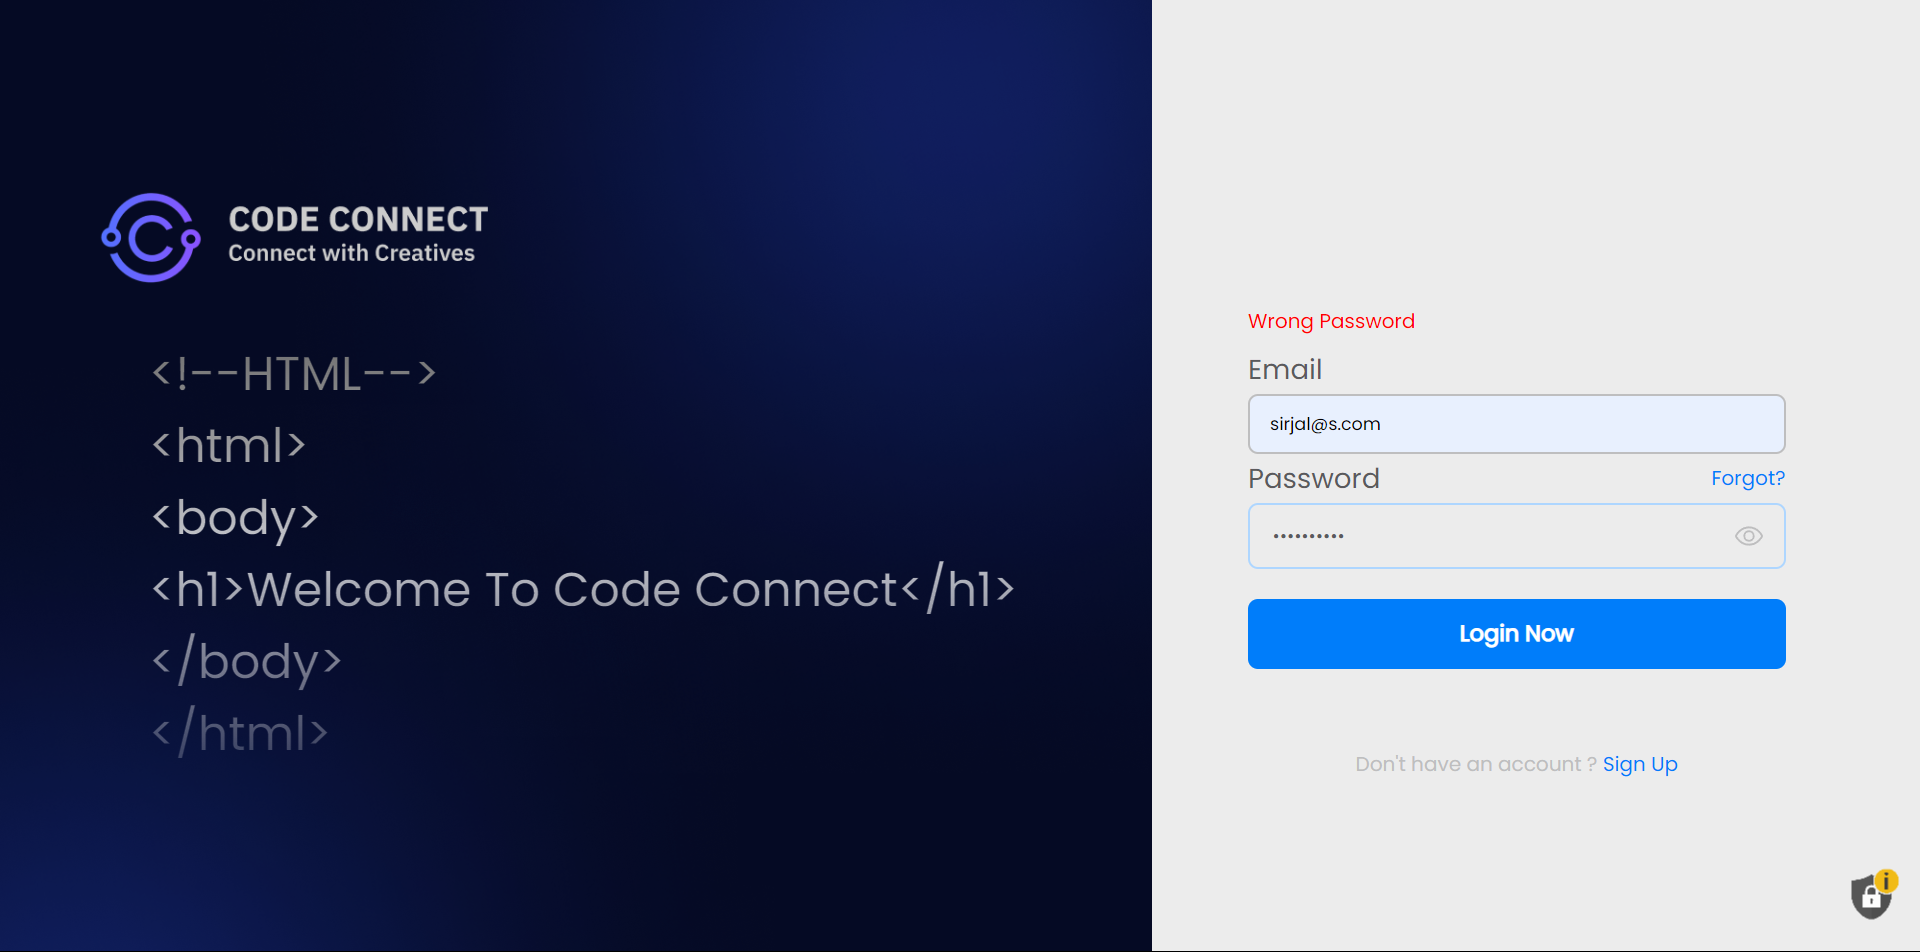
\includegraphics[width=1\textwidth]{4ImplementationAndTesting/screenshots/signin-pass-err.png}
%     \caption{Incorrect Password}
%     \label{fig: Incorrect Password}
% \end{figure}
% \begin{figure}[ht]
%     \centering
%     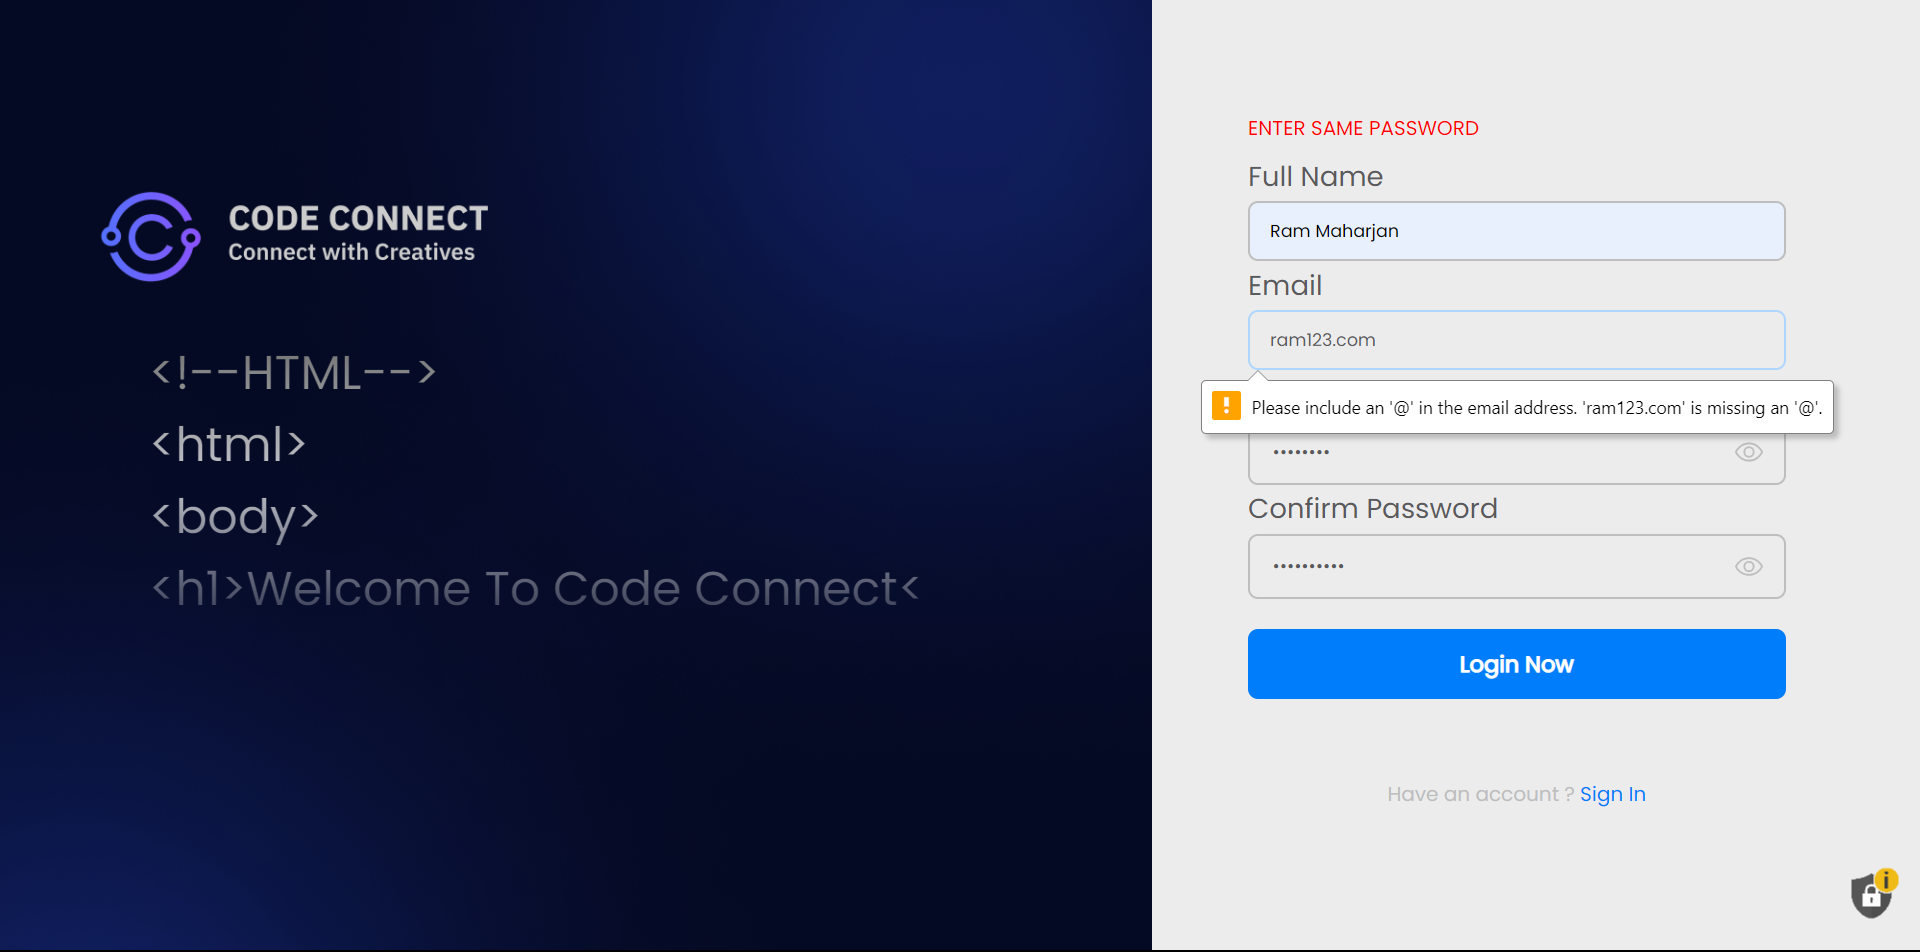
\includegraphics[width=1\textwidth]{4ImplementationAndTesting/screenshots/signup-same-pass.png}
%     \caption{Incorrect email Format In SignUp}
%     \label{fig: Incorrect email Format In SignUp}
% \end{figure}
% \begin{figure}[ht]
%     \centering
%     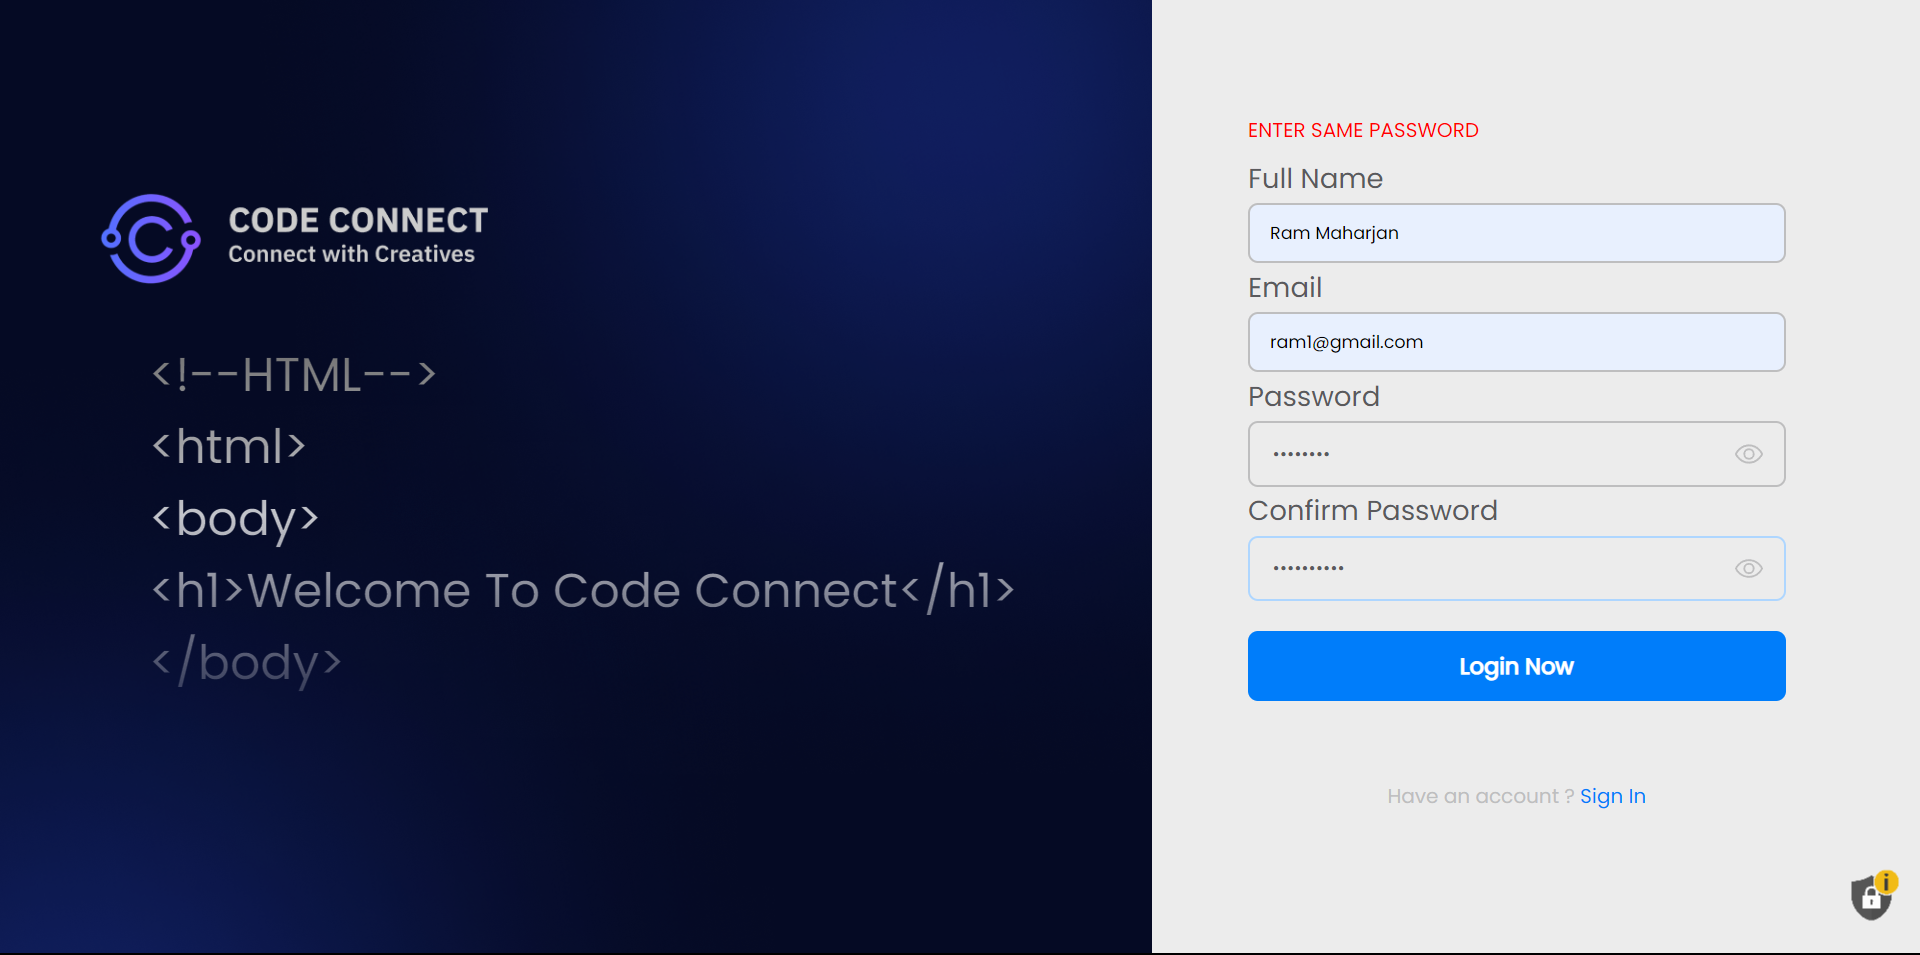
\includegraphics[width=1\textwidth]{4ImplementationAndTesting/screenshots/signup-pass-err.png}
%     \caption{Incorrect Confirm Password}
%     \label{fig: Incorrect Confirm Password}
% \end{figure}
% \begin{figure}[ht]
%     \centering
%     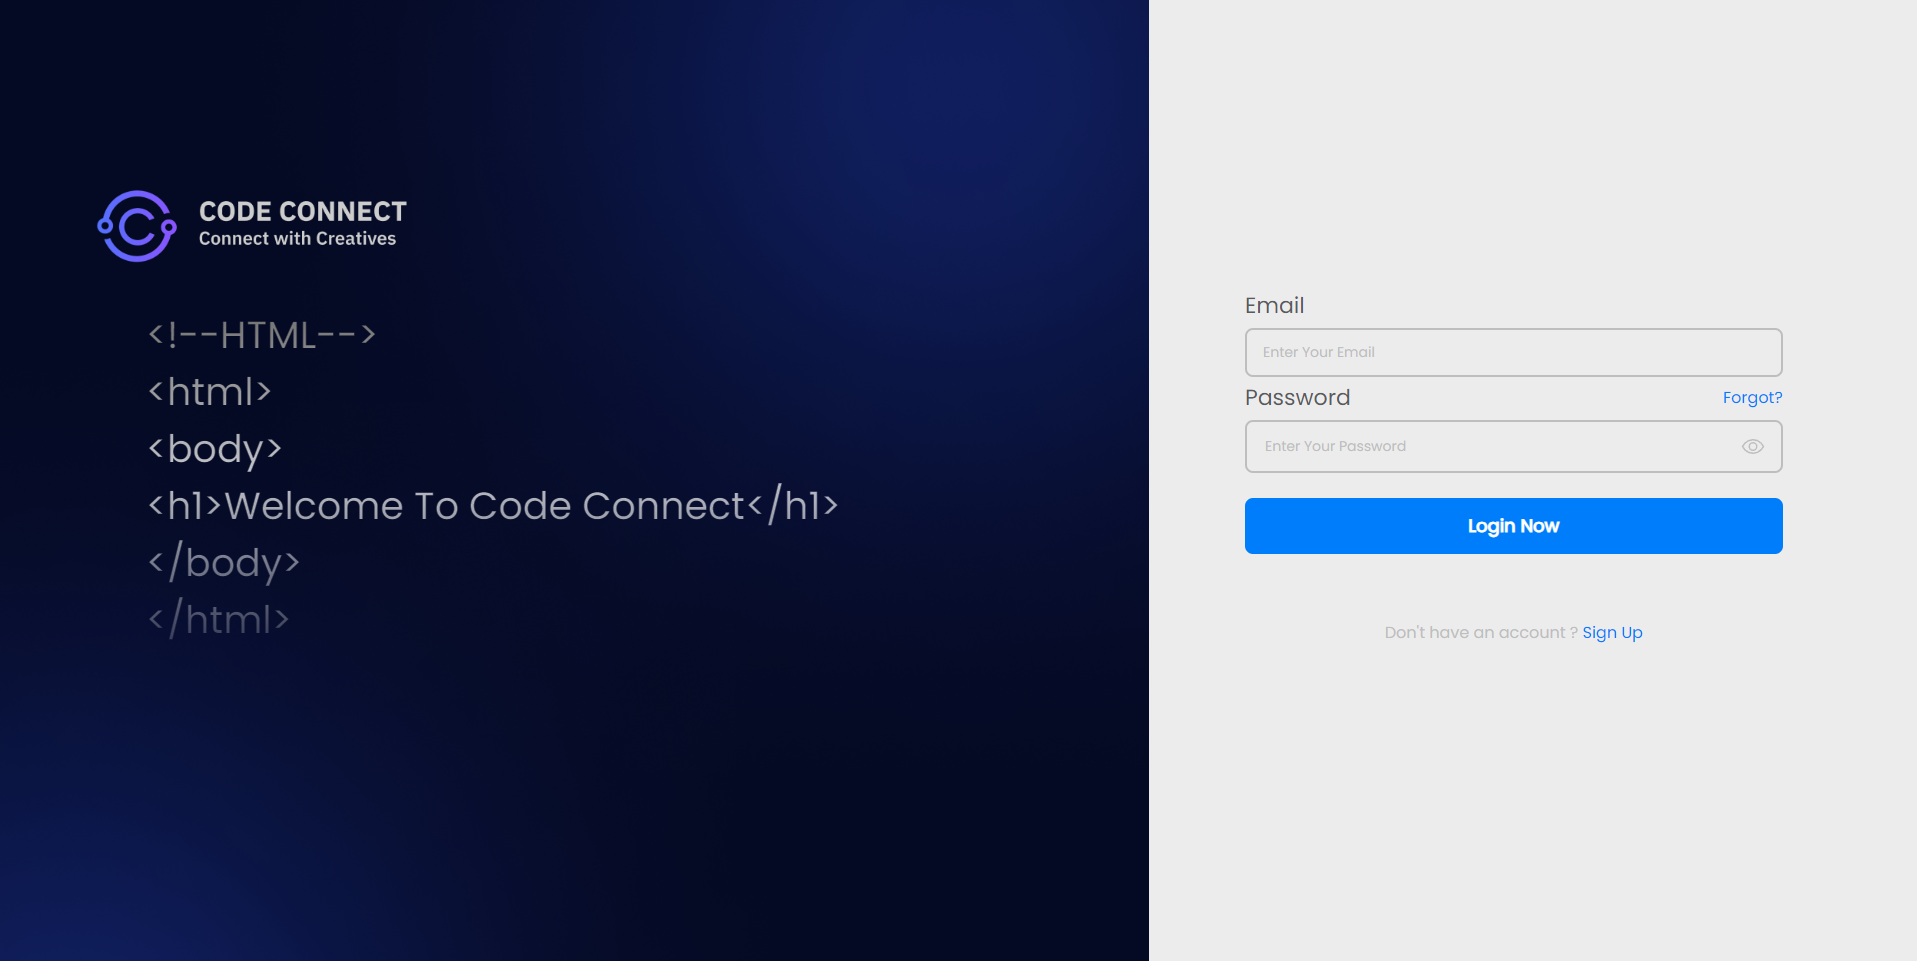
\includegraphics[width=1\textwidth]{ui_diagrams/desktop_login.png}
%     \caption{Correct SignUp Info Output}
%     \label{fig: Correct SignUp Info Output}
% \end{figure}
% \begin{figure}[ht]
%     \centering
%     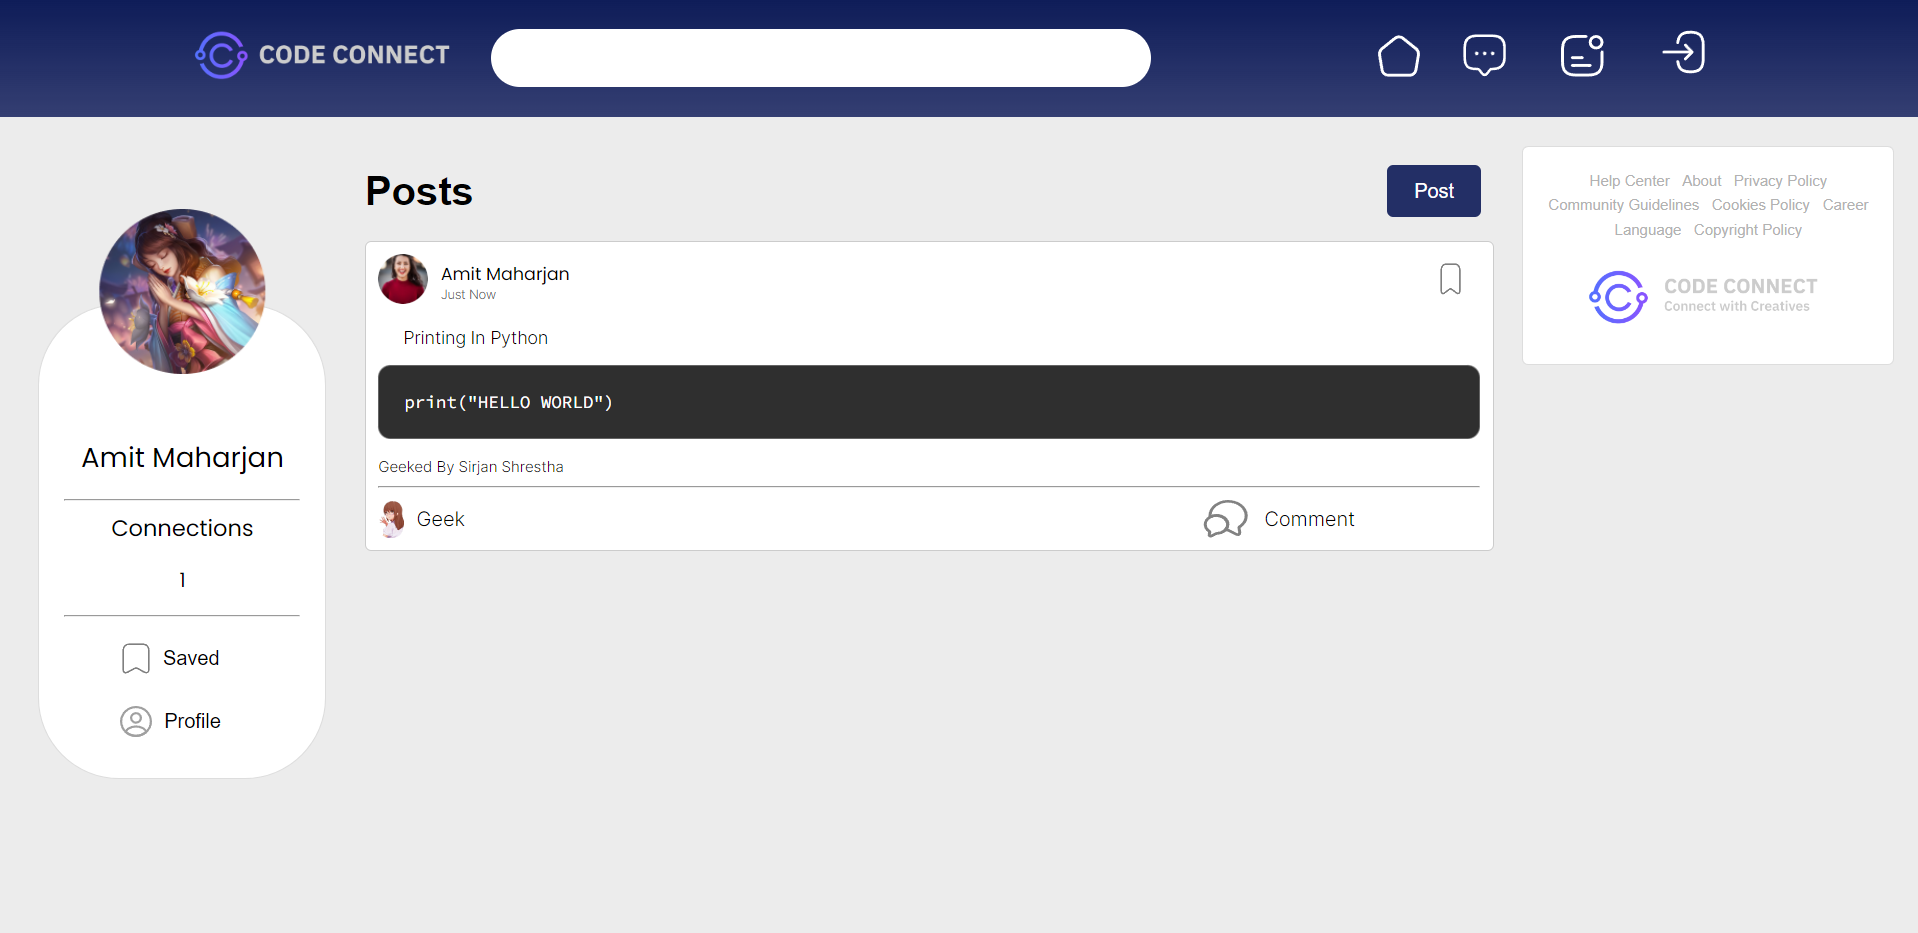
\includegraphics[width=1\textwidth]{ui_diagrams/desktop_homepage.png}
%     \caption{Correct Login Info Output}
%     \label{fig: Correct Login Info Output}
% \end{figure}

